\begin{frame}{Results and Discussion}
    \textbf{Results}\\
    \vspace{2em}
    Achieved model accuracy at first attempt without optimizations is 73.52\%.
    
    \begin{figure}[H]
        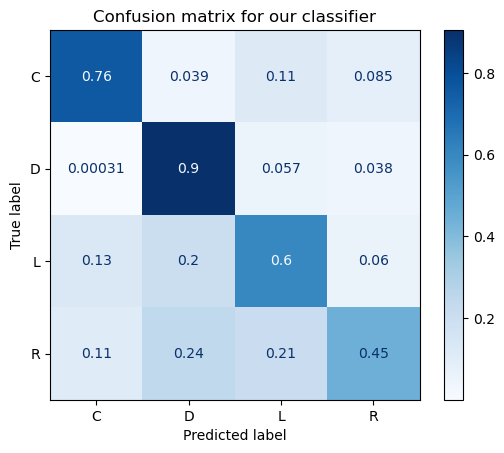
\includegraphics[width=0.6\textwidth]{matrix}
    \end{figure}
\end{frame}

\begin{frame}{Results and Discussion}
    \textbf{Accuracy of prediction per position}\\
    \vspace{2em}
    \begin{itemize}
        \item defense position (D) has 90\% accuracy
        \item center position (C) has 76\% accuracy
        \item left wing position (L) has 60\% accuracy
        \item right wing position (R) has 45\% accuracy
    \end{itemize}
\end{frame}

\begin{frame}{Results and Discussion}
    \textbf{Optimize}\\
    \vspace{2em}
    
    Model optimization should focus on areas marked with yellow and red. The worst case here is predicting right wing player position as the accuracy of it is only 45\% so it's probably more accurate to toss the coin.
    
    \begin{figure}[H]
        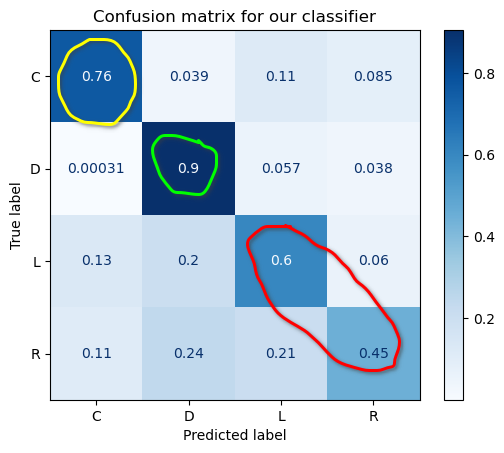
\includegraphics[width=0.55\textwidth]{optimize}
    \end{figure}
\end{frame}
